\documentclass[leqno]{article}
\usepackage[utf8x]{inputenc}
\usepackage[T1]{fontenc}
\usepackage{amsfonts}
\usepackage{enumerate}
\author{Colin Roberts}
\title{MATH 546, Homework 3}
\usepackage[left=3cm,right=3cm,top=3cm,bottom=3cm]{geometry}
\usepackage{amsmath}
\usepackage[thmmarks, amsmath, thref]{ntheorem}
%\usepackage{kbordermatrix}
\usepackage{mathtools}
\usepackage{color}
\usepackage{hyperref}
\usepackage{tikz-cd}
\usepackage{float}
\usepackage{graphicx}
\usetikzlibrary{quotes,arrows.meta}
\tikzset{
  annotated cuboid/.pic={
    \tikzset{%
      every edge quotes/.append style={midway, auto},
      /cuboid/.cd,
      #1
    }
    \draw [every edge/.append style={pic actions, densely dashed, opacity=.5}, pic actions]
    (0,0,0) coordinate (o) -- ++(-\cubescale*\cubex,0,0) coordinate (a) -- ++(0,-\cubescale*\cubey,0) coordinate (b) edge coordinate [pos=1] (g) ++(0,0,-\cubescale*\cubez)  -- ++(\cubescale*\cubex,0,0) coordinate (c) -- cycle
    (o) -- ++(0,0,-\cubescale*\cubez) coordinate (d) -- ++(0,-\cubescale*\cubey,0) coordinate (e) edge (g) -- (c) -- cycle
    (o) -- (a) -- ++(0,0,-\cubescale*\cubez) coordinate (f) edge (g) -- (d) -- cycle;
    \path [every edge/.append style={pic actions, |-|}]
    (b) +(0,-5pt) coordinate (b1) edge ["\cubex \cubeunits"'] (b1 -| c)
    (b) +(-5pt,0) coordinate (b2) edge ["\cubey \cubeunits"] (b2 |- a)
    (c) +(3.5pt,-3.5pt) coordinate (c2) edge ["\cubez \cubeunits"'] ([xshift=3.5pt,yshift=-3.5pt]e)
    ;
  },
  /cuboid/.search also={/tikz},
  /cuboid/.cd,
  width/.store in=\cubex,
  height/.store in=\cubey,
  depth/.store in=\cubez,
  units/.store in=\cubeunits,
  scale/.store in=\cubescale,
  width=1,
  height=1,
  depth=1,
  units=,
  scale=2,
}

\theoremstyle{nonumberplain}
\theoremheaderfont{\itshape}
\theorembodyfont{\upshape:}
\theoremseparator{.}
\theoremsymbol{\ensuremath{\square}}
\newtheorem{proof}{Proof}
\theoremsymbol{\ensuremath{\square}}
\newtheorem{lemma}{Lemma}
%\theoremsymbol{\ensuremath{\square}}
\newtheorem{solution}{Solution}
%\theoremseparator{. ---}
%\theoremsymbol{\mbox{\texttt{;o)}}}
%\newtheorem{varsol}{Solution (variant)}

\newcommand{\id}{\mathrm{Id}}
\newcommand{\im}{\mathrm{im}}
\newcommand{\R}{\mathbb{R}}
\newcommand{\N}{\mathbb{N}}
\newcommand{\Z}{\mathbb{Z}}
\newcommand{\C}{\mathbb{C}}
\newcommand{\RE}{\textrm{Re}}
\newcommand{\IM}{\textrm{Im}}

\newcommand{\End}{\mathrm{End}}

% Matlab code
\usepackage{listings}
\usepackage{color} %red, green, blue, yellow, cyan, magenta, black, white
\definecolor{mygreen}{RGB}{28,172,0} % color values Red, Green, Blue
\definecolor{mylilas}{RGB}{170,55,241}

\begin{document}
\maketitle
\begin{large}
\begin{center}
Solutions
\end{center}
\end{large}

%%%%%%%%%%%%%%%%%%%%%%%%%%%%%%%%%%%%%%%%%%%%%%%%%%%%%%%%%%%%%%%%%%%%%%%%%%%%%%%%%%%%%%%%%%%%%%%%%%%%%%%%%%%%%%%%%%%%%
%%%%%%%%%%%%%%%%%%%%%%%%%PROBLEM%%%%%%%%%%%%%%%%%%%%%%%%%%%%%%%%%%%%%%%%%%%%%%%%%%%%%%%%%%%%%%%%%%%%%%%%%%%%%%%%%%%%%%%%%%%%%%%%%%%%%%%%%%%%%%%%%%%%%%%%%%%%%%%%%%%%%%%%%%%%%%%%%%%%%%%%%%%%%%%%%%%%%%%%%%%%%%%%%%%%%%%%%%%%%%%%%%%%%%%%%%

\paragraph{Problem 1 (Weak solutions and strong solutions).}
In class, we have discussed that if you have a weak solution of the
Laplace equation, then it is also a strong solution assuming that it
is smooth enough to allow for certain operations. In other words,
assume that you have a function $u\in H^1_g$ so that
\begin{align*}
  \int_\Omega \nabla u \cdot \nabla v
  =
  \int_\Omega f v
  +
  \int_{\Gamma_N} h v
  \qquad\qquad \forall v\in H^1_0,
\end{align*}
and that serendipitously this function is in fact also in
$C^2(\Omega)$. Then you can integrate by parts to see that for this
function we have that
\begin{align*}
  \int_\Omega (-\Delta u - f) v
  +
  \int_{\Gamma_N} \left(\frac{\partial u}{\partial n} - h \right) v
  \qquad\qquad \forall v\in H^1_0.
\end{align*}
We argued in class that this implies that $-\Delta u - f=0$ in a
pointwise sense assuming that $f\in C^0(\Omega)$.

Complete the argument to show that also $\frac{\partial u}{\partial n}
- h=0$ pointwise assuming that $h\in C^0(\Gamma_N)$. The argument is
not difficult, so pay attention to 
justifying why each step is correct and why each operation is in fact
allowed for all of the functions you are considering in your argument.

\begin{solution}
Since we have that
\[
-\Delta u - f=0
\]
pointwise, we have that
\[
\int_{\Gamma_N} \left( \frac{\partial u}{\partial n} - h\right)v =0
\]
for all $v\in H_0^1.$  We can specifically choose that $v=\frac{\partial u}{\partial n}-h$.  Why is this okay? Well, since $u\in C^2(\Omega)$ we have that $\frac{\partial u}{\partial n} \in H^1_0$ and that $h\in C^0(\Gamma_N)$ implies that $h\in H^1_0$ since $h$ must be bounded and continuous.  Then, with this $v$, we have
\[
\int_{\Gamma_N} \left(\frac{\partial u}{\partial n} - h\right)^2 = 0
\]
which means that we have 
\[
\frac{\partial u}{\partial n}-h = 0 ~~\textrm{almost everywhere.}
\]
Since we also have that $u\in C^2(\Omega)$ we have that $\frac{\partial u}{\partial n} \in C^0(\Gamma_n)$ which means that
\[
\frac{\partial u}{\partial n}-h \in C^0(\Gamma_N).
\]
But, since this function is in $C^0(\Gamma_N)$ and is zero almost everywhere, it must be in fact zero everywhere.  

To see this, assume that at some point it was not zero, then by continuity there would be an open neighborhood about that point in which 
\[
\frac{\partial u}{\partial n}-h \neq 0.
\]
This open neighborhood then has nonzero measure, and this contradicts the fact that we found 
\[
\frac{\partial u}{\partial n}-h = 0 ~~\textrm{pointwise.}
\]
So, we have that 
\[
\frac{\partial u}{\partial n}-h = 0 ~~\textrm{almost everywhere.}
\]
\end{solution}
\pagebreak



\paragraph{Problem 2 (The biharmonic equation).}
The biharmonic equation is a model for the deformation of thin
two-dimensional structures such as stadium roofs. In its simplest form
it looks like this:
\begin{align*}
  \Delta\Delta u &= f 
  \qquad\qquad && \text{in $\Omega$},
  \\
  u &= g  && \text{on $\partial\Omega$},
  \\
  \frac{\partial u}{\partial n} &= h  && \text{on $\partial\Omega$}.
\end{align*}
(This is a fourth order differential equation, so it needs twice as
many boundary conditions as the Laplace equation and so we are
prescribing here both Dirichlet and Neumann conditions for the
solution.)

For many of the same reasons as for the Laplace equation, it is not
possible to always find strong solutions to this equation. Retrace
the steps we discussed when we derived the weak formulation of the
Laplace equation to obtain a weak formulation of the biharmonic
equation.

Then also go through the steps of Question 1 to identify what the
appropriate function spaces for the (weak) solution $u$ and the test
functions $v$ should be. Recall how we argued what the boundary values
for the test function needed to be for the Laplace equation, and think
about what that would mean in the current context; specifically, you
will want to incorporate \textit{both} boundary conditions above into
the spaces for $u$ and $v$.

\begin{solution}
We could start with a variational method to arrive at this equation (which I do like), or we can move from this strong form to the weak form.  The latter is how I'll do this, but the fact is that if we start with the variational method, $v$ must be zero almost everywhere on the boundary since $(u+\epsilon v)\vert_{\partial \Omega}=g$ almost everywhere. That is, $v$ is in the tangent space ($X_0$) to what ever function space $X_g$ that $u$ is in. Hopefully just saying this is a good enough argument given that we spent the time discussing this in 620!

Given that, we can now say we take a test function $v$, and ``weaken" our strong PDE by forcing
\[
\int_\Omega (\Delta \Delta u)v = \int_\Omega fv.
\]
We can integrate by parts
\begin{align*}
    \int_\Omega (\Delta \Delta u)v &= \int_\Omega fv\\
    \iff~ - \int_\Omega (\nabla (\Delta u))\cdot \nabla v + \int_{\partial \Omega} (\nabla (\Delta u)\cdot n) v &= \int_\Omega fv,
\end{align*}
and note that
\[
\int_{\partial \Omega} (\nabla (\Delta u)\cdot n) v =0
\]
since $v\in X_0$ (i.e., has zero boundary values almost everywhere). Then
\begin{align*}
    -\int_\Omega (\nabla (\Delta u))\cdot \nabla v &= \int_\Omega fv\\
    \iff ~ (\Delta u) (\Delta v) - \int_{\partial \Omega} (\Delta u)(\nabla v \cdot n) &= \int_\Omega fv
\end{align*}
and note that we again have
\[
\int_{\partial \Omega} (\Delta u)(\nabla v \cdot n) = 0
\]
since $v$ is zero almost everywhere on the boundary.  Thus we arrive at
\[
\int_\Omega (\Delta u)(\Delta v) = \int_\Omega fv.
\]
Now we can see that we require $u$ to have two weak derivatives, to be square integrable, and that $u$ is equal to $g$ along the boundary.  So, we can say that $u\in H^2_g$.  However, we also require that $u$ has Neumann boundary info, and this means specifically that
\[
u \in \left\{ H^2_g ~\left\vert~ \frac{\partial u}{\partial n}\right. = h ~ \textrm{on $\partial \Omega$}\right\}.
\]
Then, we also notice that $v$ must have to have two weak derivatives but has zero boundary values (almost everywhere) since $v$ is a variation.  So we have $v\in H^2_0$. 

At some point will we make the argument that $C^\infty_0$ functions are dense in (some) of these spaces?  I think I've seen this before at other points since I've heard of people referring to test functions as $C^\infty_0$ functions. 

Also, if you wanted to see this done from the variational method, I could work that out for you.  It seemed to me that this is what you wanted to see, though.  In that case, you define a functional
\[
I[u] = \int_\Omega \frac{1}{2} \| \Delta u\|
\]
and find where the variation of this functional is zero and show that it is actually a minimizer.
\end{solution}
\pagebreak

\paragraph{Problem 3 (Singular solutions of the biharmonic equation).}
Recall how we showed that solutions of the Laplace equation may not
always be in $C^2$ by considering the case of a domain with a
reentrant corner (namely, a sector with an opening angle greater than
$\pi$).

Do the same argument for solutions of the biharmonic equation with
$f=0$. Ideally, one would of course like to have strong solutions
$u\in C^4$. Show that in a circular sector with a reentrant corner,
this is not always possible by explicitly constructing a solution of
the equation. For the Laplace equation, we choose $g=0$ along the two
lines adjacent to the troublesome corner. This should also work here,
and you should think about whether you can also choose $h=0$. If you
can't, make sure that $g$ and $h$ are at the very least
continuous functions.

\begin{solution}
Let $\Omega$ be the ``Pac-Man" shaped region (the region with a reentrant corner) where our angle is $\theta$.
\begin{figure}[h]
    \centering
    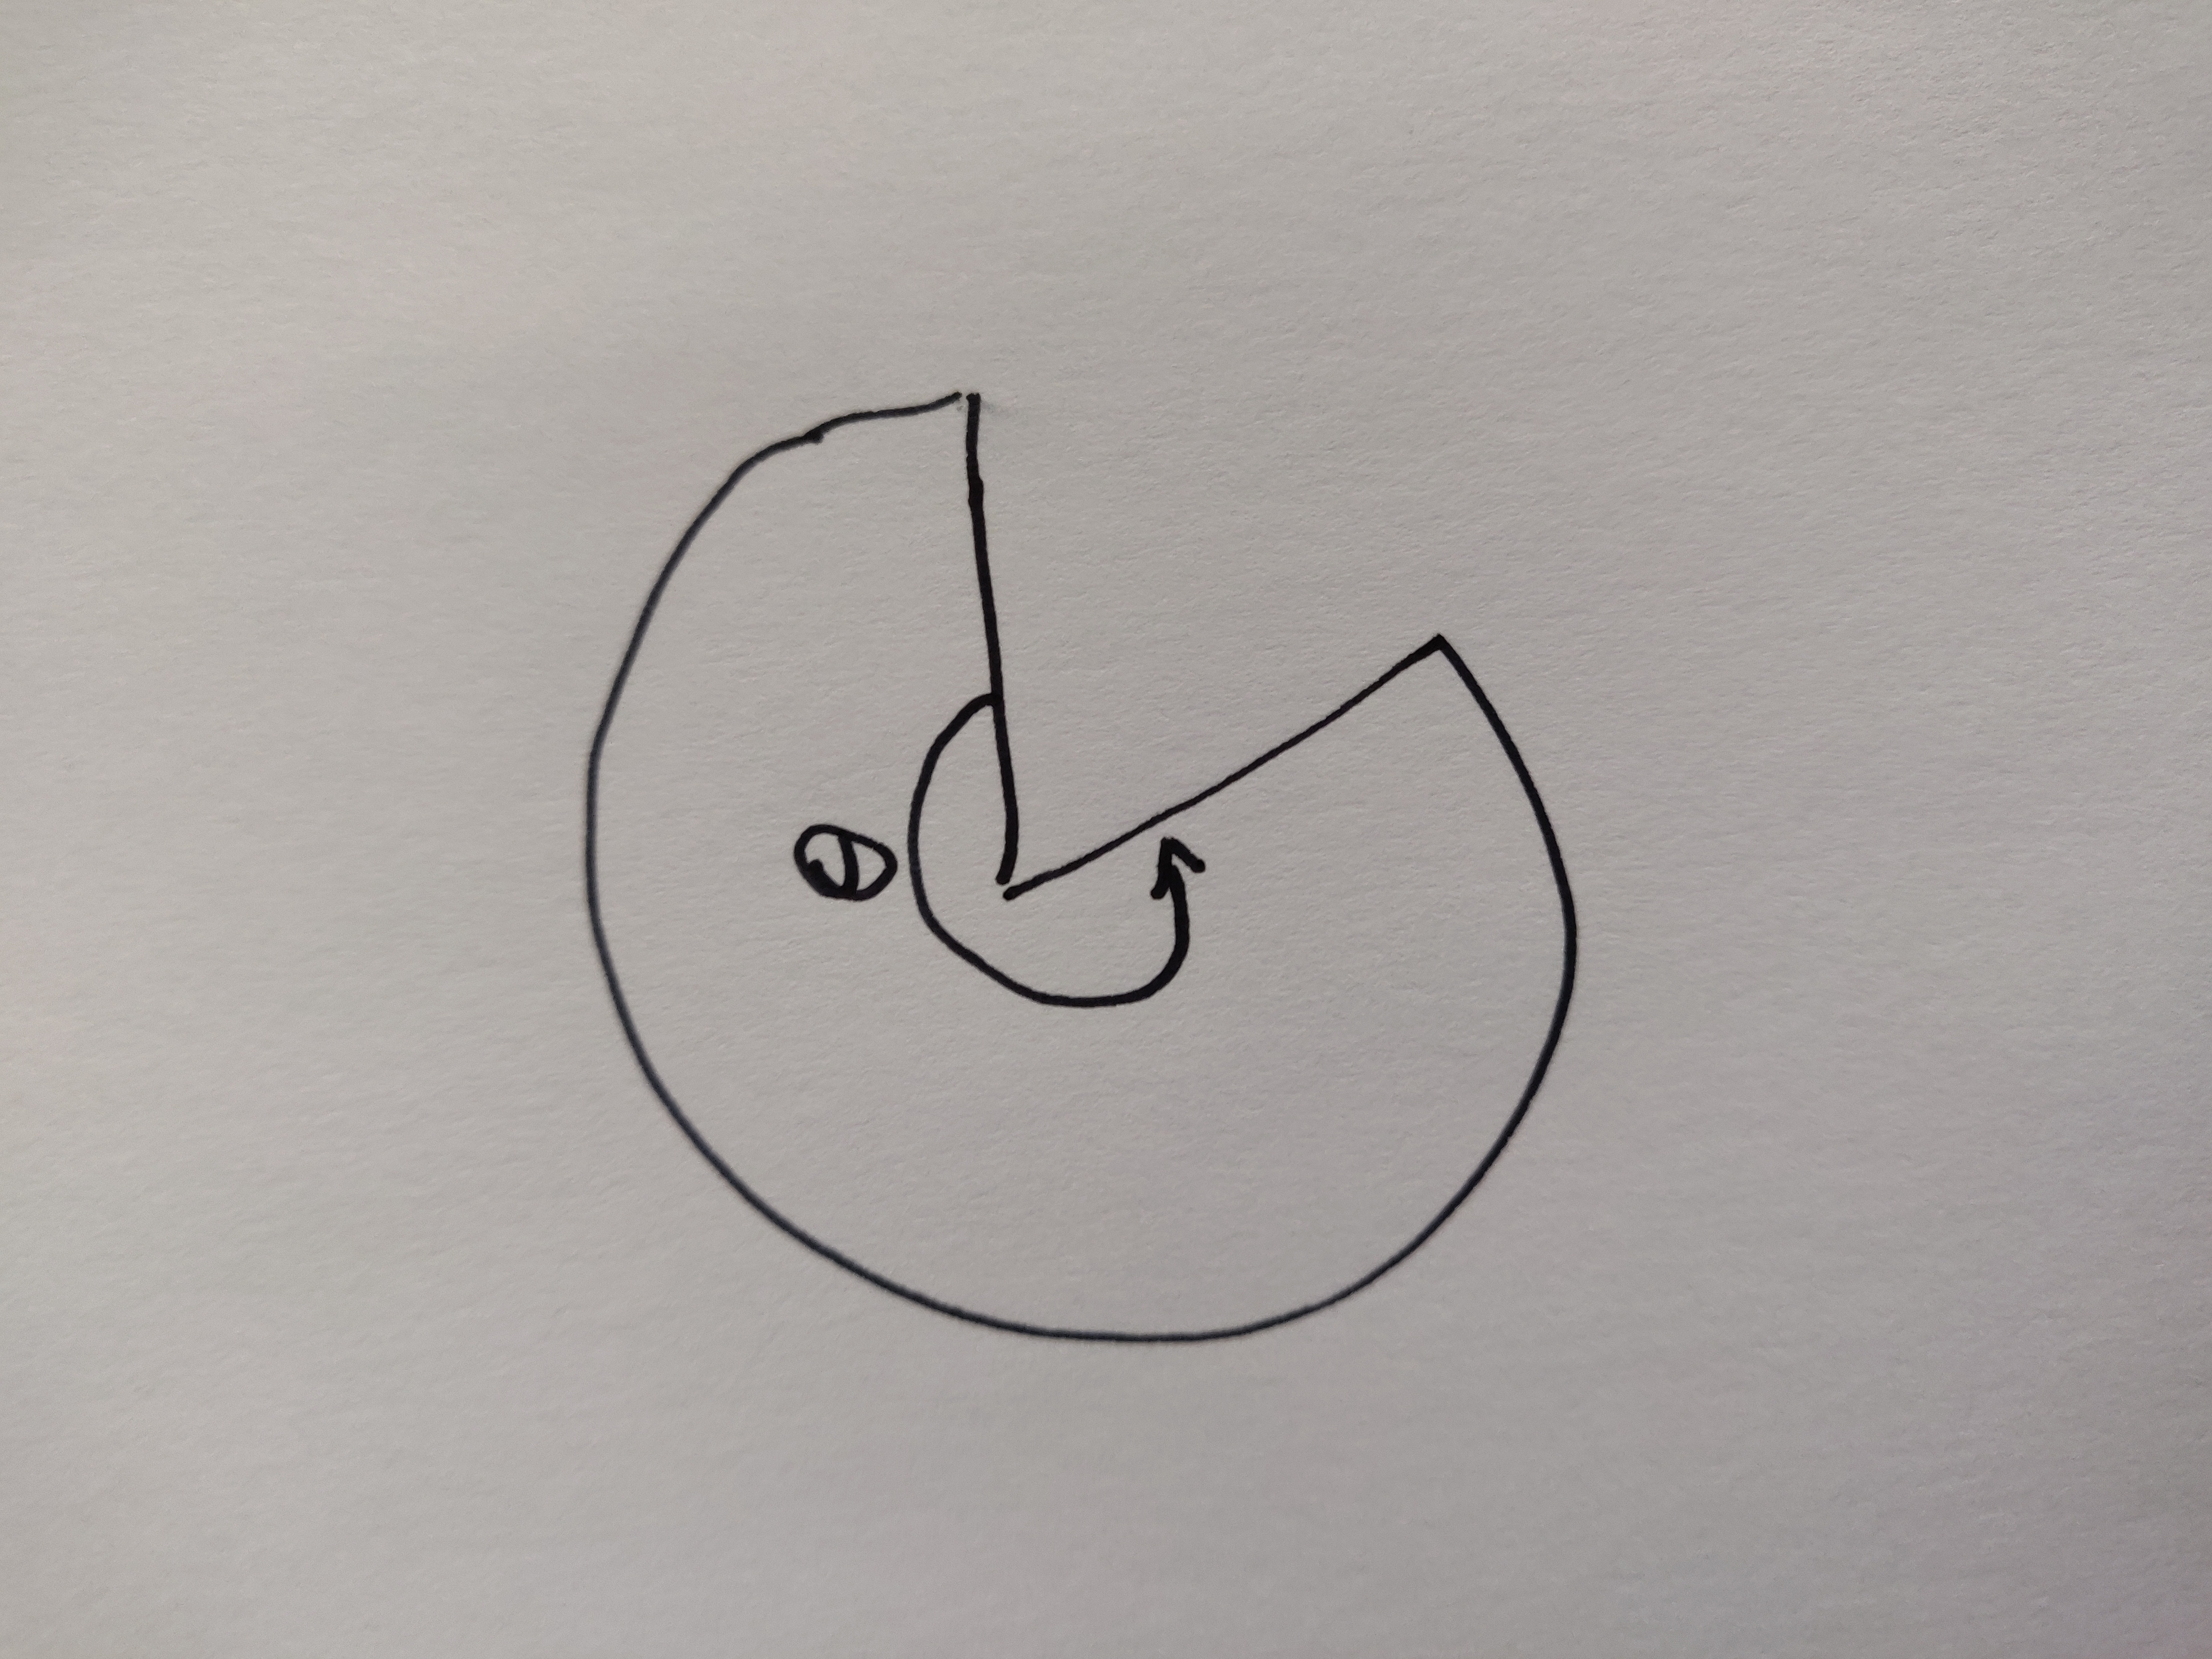
\includegraphics[width=.4\textwidth]{IMG_20190404_165308.jpg}
    \caption{Caption}
    \label{fig:my_label}
\end{figure}
Note that 
\[
u(r,\phi) = r^\alpha \sin (k\phi)
\]
is a solution to the biharmonic equation $\Delta \Delta u = 0$.  So, we take this, and we have
\begin{align*}
    \Delta \Delta u(r,\phi) &= \Delta (\alpha^2-k^2)r^{\alpha -2} \sin(k \phi)\\
    &= (\alpha^2-k^2)((\alpha-2)^2-k^2)\sin(k\phi).
\end{align*}
Now, take the case where $g=0$, then we have that $k=n\frac{\pi}{\theta}$ for $n\in \N$. This means that
\[
\alpha = \pm n\frac{\pi}{\theta}, ~\pm n\frac{\pi}{\theta}+2
\]
for $n\in \N$.  Then we have that
\begin{align*}
\left.\frac{\partial u}{\partial n} \right\vert_{\phi=\frac{\pi}{\theta}} &= \left[\frac{1}{r}\frac{\partial }{\partial \phi}r^{n\frac{\pi}{\theta}}\sin\left(n\frac{\pi}{\theta}\phi\right)\right]_{\phi=\frac{\pi}{\theta}}\\
&= n\frac{\pi}{\theta}r^{n\frac{\pi}{\theta}-1}
\end{align*}
So we can let
\[
h=\frac{\pi}{\theta}r^{\frac{\pi}{\theta}-1}
\]
which gives $n=1$ and our solution becomes
\[
u(r,\phi) = r^{\frac{\pi}{\theta}}\sin\left(\frac{\pi}{\theta}\phi\right)
\]
Note that this solution is not in $C^4$ since we have that
\[
\frac{\partial^3}{\partial r^3} u(r,\phi) = \frac{\pi}{\theta} \left( \frac{\pi}{\theta}-1\right) \left( \frac{\pi}{\theta}-2\right) r^{\frac{\pi}{\theta}-3} \sin\left(\frac{\pi}{\theta} \phi \right).
\]
Then we can isolate part of the $C^3$ norm since
\begin{align*}
    \|u\|_{C^3}\leq \int_\Omega \|\nabla^3 u\| &\leq \int_\Omega \left|\frac{\partial^3}{\partial r^3} u(r,\phi)\right|
\end{align*}
and that we find
\begin{align*}
\int_\Omega \left|\frac{\partial^3}{\partial r^3} u(r,\phi)\right| &\propto \int_0^R r^{\frac{\pi}{\theta}-3} r dr\\
&= \int_0^R r^{\frac{\pi}{\theta}-2} dr = \infty
\end{align*}
since $\frac{\pi}{\theta}-2 < -1$. So since $u(r,\phi) \notin C^3$, we also have that $u(r,\phi)\notin C^4$. 


If $h=0$, then we must have that $n\frac{\pi}{\theta}=0$, and so our only solution is zero almost everywhere. So this seems to limit what boundary conditions we can assign on the outer portion of our domain (the $r=R$ boundary).


 

\end{solution}
\pagebreak


\paragraph{Problem 4 (Singular solutions of the Stokes equations).}
For both the Laplace equation and the biharmonic equation (in the
previous problem), we have constructed solutions that have a
singularity (i.e., for which $u\not\in C^2$ or $u\not\in C^4$,
respectively), but at least the solution remained bounded -- it was
just that some derivative ``blows up''.

But not even this has to always be true. It's just a matter of how
many derivatives you have on a variable once you're in the weak
formulation. Take, for example, the Stokes equations
\begin{align*}
  -\Delta \mathbf u(\mathbf x) + \nabla p(\mathbf x) &= \mathbf f(\mathbf x),
  \\
  -\nabla\cdot \mathbf u(\mathbf x) &= 0.
\end{align*}
For this equation, you derived a weak formulation in the previous
homework, which will have looked something like this:
\begin{align*}
  \int_\Omega \nabla \mathbf u : \nabla \mathbf v
  -
  \int_\Omega p (\nabla \cdot \mathbf v)
  -
  \int_\Omega (\nabla\cdot \mathbf u) q
  &=
  \int_\Omega \mathbf v \cdot \mathbf v,
\end{align*}
for all test functions $\mathbf v \in H^1_0(\Omega)^3, q\in
L^2(\Omega)$, where I have purposefully neglected all boundary
terms. (Forgetting about boundary terms is correct if one enforces
Dirichlet boundary conditions on $\mathbf u$, though one then also
needs $\mathbf v\in H^1_0(\Omega)^3$; one also gets complications with
non-uniqueness of the pressure component of the solution -- all
reasons why we don't want to deal too much with details of boundary terms here.)

The point to observe here is that neither derivatives of the pressure
$p$ nor of the test function $q$ appear in the weak formulation. So
one may suspect that these functions only need to be in $L^2$ and
that, consequently, they can have worse singularities than the
solutions of the Laplace and biharmonic equations, for which first and
second weak derivatives appear in the weak formulation.

Here is a situation you may want to consider -- called the
``lid-driven'' or simply the ``driven cavity'' (because as you will
see in a second, a lid ``drives'' the motion of the fluid): Take a box
(or in 2d a rectangle) filled with a viscous fluid -- the
``cavity''. The sides of the box are fixed, but the top of the box is
a plate larger than the box that is sliding across the box at a
constant velocity. Since it is in contact with the fluid, the viscous
friction between the top and the fluid drags the fluid along.

Try to concisely describe in formulas the boundary conditions you have for this physical
situation. Now consider the 2d case and specifically the places where
the sliding top is in contact with the fixed sides -- i.e., the top
left and top right corners of the box. At these locations, the fluid
dragged along by the sliding top encounters a fixed wall, and so has
to change its direction of flow.

Without having to explicitly construct a solution as a closed-form
expression, can you speculate what the pressure needs to do in (the
vicinity of) these
corners for all boundary conditions to be satisfied exactly? Using
your physical intuition of what a pressure really is (namely, a kind of
\textit{force density}), do you think that the pressure should remain bounded
from above and/or below in each of these corners, or do you think that
it might go to plus or minus infinity?

\begin{solution}
Let's picture the cube as having length, width, and height all equal to 1.  We can place this in $\R^3$ such that the one vertex lies at $(0,0,0)$ and its apposing vertex is at $(1,1,1)$.  

\begin{center}
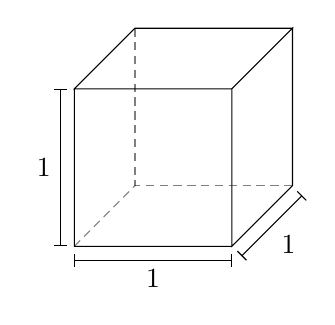
\begin{tikzpicture}
  \pic {annotated cuboid};
\end{tikzpicture}
\end{center}

Then we can define the boundary conditions on the different faces
\begin{align*}
    \Gamma_1 &= \{ (x,y,z) ~\vert~ x,y \in [0,1] ~\textrm{and}~ z=0\}\\
    \Gamma_2 &= \{ (x,y,z) ~\vert~ x \in [0,1], ~y=0,  ~\textrm{and}~ z\in (0,1]\}\\
    \Gamma_3 &= \{ (x,y,z) ~\vert~ x \in [0,1], ~y=1,  ~\textrm{and}~ z\in (0,1]\}\\
    \Gamma_4 &= \{ (x,y,z) ~\vert~ x=0 , ~y\in [0,1],  ~\textrm{and}~ z\in (0,1]\}\\
    \Gamma_5 &= \{ (x,y,z) ~\vert~ x=1, ~y\in [0,1],  ~\textrm{and}~ z\in (0,1]\}\\
    \Gamma_6 &= \{ (x,y,z) ~\vert~ x, \in (0,1), ~\textrm{and}~ z=1\}.
\end{align*}
Then the boundary conditions we assign are
\[
\mathbf{u} = \mathbf{0} ~\textrm{on $\Gamma_i$, for $i=1,2,3,4,5$},
\]
since the fluid cannot move at the boundary.  Then, letting $\mathbf{w}$ be the velocity of the lid on the top (which should only move along the surface, i.e., $\mathbf{w}=(w_1,w_2,0)$), we also have
\[
\mathbf{u}= \mathbf{w} ~\textrm{ on $\Gamma_6$}.
\]

There are apparent issues at the corners along the top.  Why?  Well, imagine a single particle in the fluid that is very close to the lid so that its velocity is essentially $\mathbf{w}$.  More rigorously, we can say that for some any $0<\epsilon \ll 1$ there is a particle near lid (that is, $z=(1-\delta)$ and some $0<\delta\ll 1$) that will be traveling with velocity $(1-\epsilon)\mathbf{w}$. However if this particle is also near one of the walls of the container, say $y$ component very close to $1$, the velocity of this particle will have to rapidly change direction as the particle cannot pass through this boundary.  This rapid change in direction happens over an arbitrarily small distance and if we consider the work done
\[
W=\mathbf{F}\cdot \mathbf{d}
\]
(which for small displacements $\mathbf{d}$ is accurate), the work will be fixed while we can shrink the displacement $\|\mathbf{d}\|$ as small as we would like.  Roughly speaking, if $W=1$, and $\|d\|=\varepsilon$, then
\[
\|F\|\approx \frac{1}{\varepsilon}.
\]
This seems to say that the force, although finite at any chosen point, can be as large as we want it to be.

Given this argument, it seems like the pressure near the corners will be unbounded.  However, I'd imagine that it must be unbounded in some way so that when integrated over, the value is finite.  If not, then there would be some region where the force itself is infinite and that is unphysical.

Below is a picture of what I'm trying to describe.  Hopefully it helps some! (It's on the next page)
\begin{figure}
    \centering
    \includegraphics[width=.7\textwidth]{IMG_20190404_164742.jpg}
\end{figure}

\end{solution}




\pagebreak





\end{document}



